% Options for packages loaded elsewhere
\PassOptionsToPackage{unicode}{hyperref}
\PassOptionsToPackage{hyphens}{url}
\PassOptionsToPackage{dvipsnames,svgnames,x11names}{xcolor}
%
\documentclass[
  letterpaper,
  DIV=11,
  numbers=noendperiod]{scrartcl}

\usepackage{amsmath,amssymb}
\usepackage{iftex}
\ifPDFTeX
  \usepackage[T1]{fontenc}
  \usepackage[utf8]{inputenc}
  \usepackage{textcomp} % provide euro and other symbols
\else % if luatex or xetex
  \usepackage{unicode-math}
  \defaultfontfeatures{Scale=MatchLowercase}
  \defaultfontfeatures[\rmfamily]{Ligatures=TeX,Scale=1}
\fi
\usepackage{lmodern}
\ifPDFTeX\else  
    % xetex/luatex font selection
\fi
% Use upquote if available, for straight quotes in verbatim environments
\IfFileExists{upquote.sty}{\usepackage{upquote}}{}
\IfFileExists{microtype.sty}{% use microtype if available
  \usepackage[]{microtype}
  \UseMicrotypeSet[protrusion]{basicmath} % disable protrusion for tt fonts
}{}
\makeatletter
\@ifundefined{KOMAClassName}{% if non-KOMA class
  \IfFileExists{parskip.sty}{%
    \usepackage{parskip}
  }{% else
    \setlength{\parindent}{0pt}
    \setlength{\parskip}{6pt plus 2pt minus 1pt}}
}{% if KOMA class
  \KOMAoptions{parskip=half}}
\makeatother
\usepackage{xcolor}
\ifLuaTeX
  \usepackage{luacolor}
  \usepackage[soul]{lua-ul}
\else
  \usepackage{soul}
  
\fi
\setlength{\emergencystretch}{3em} % prevent overfull lines
\setcounter{secnumdepth}{-\maxdimen} % remove section numbering
% Make \paragraph and \subparagraph free-standing
\makeatletter
\ifx\paragraph\undefined\else
  \let\oldparagraph\paragraph
  \renewcommand{\paragraph}{
    \@ifstar
      \xxxParagraphStar
      \xxxParagraphNoStar
  }
  \newcommand{\xxxParagraphStar}[1]{\oldparagraph*{#1}\mbox{}}
  \newcommand{\xxxParagraphNoStar}[1]{\oldparagraph{#1}\mbox{}}
\fi
\ifx\subparagraph\undefined\else
  \let\oldsubparagraph\subparagraph
  \renewcommand{\subparagraph}{
    \@ifstar
      \xxxSubParagraphStar
      \xxxSubParagraphNoStar
  }
  \newcommand{\xxxSubParagraphStar}[1]{\oldsubparagraph*{#1}\mbox{}}
  \newcommand{\xxxSubParagraphNoStar}[1]{\oldsubparagraph{#1}\mbox{}}
\fi
\makeatother

\usepackage{color}
\usepackage{fancyvrb}
\newcommand{\VerbBar}{|}
\newcommand{\VERB}{\Verb[commandchars=\\\{\}]}
\DefineVerbatimEnvironment{Highlighting}{Verbatim}{commandchars=\\\{\}}
% Add ',fontsize=\small' for more characters per line
\usepackage{framed}
\definecolor{shadecolor}{RGB}{241,243,245}
\newenvironment{Shaded}{\begin{snugshade}}{\end{snugshade}}
\newcommand{\AlertTok}[1]{\textcolor[rgb]{0.68,0.00,0.00}{#1}}
\newcommand{\AnnotationTok}[1]{\textcolor[rgb]{0.37,0.37,0.37}{#1}}
\newcommand{\AttributeTok}[1]{\textcolor[rgb]{0.40,0.45,0.13}{#1}}
\newcommand{\BaseNTok}[1]{\textcolor[rgb]{0.68,0.00,0.00}{#1}}
\newcommand{\BuiltInTok}[1]{\textcolor[rgb]{0.00,0.23,0.31}{#1}}
\newcommand{\CharTok}[1]{\textcolor[rgb]{0.13,0.47,0.30}{#1}}
\newcommand{\CommentTok}[1]{\textcolor[rgb]{0.37,0.37,0.37}{#1}}
\newcommand{\CommentVarTok}[1]{\textcolor[rgb]{0.37,0.37,0.37}{\textit{#1}}}
\newcommand{\ConstantTok}[1]{\textcolor[rgb]{0.56,0.35,0.01}{#1}}
\newcommand{\ControlFlowTok}[1]{\textcolor[rgb]{0.00,0.23,0.31}{\textbf{#1}}}
\newcommand{\DataTypeTok}[1]{\textcolor[rgb]{0.68,0.00,0.00}{#1}}
\newcommand{\DecValTok}[1]{\textcolor[rgb]{0.68,0.00,0.00}{#1}}
\newcommand{\DocumentationTok}[1]{\textcolor[rgb]{0.37,0.37,0.37}{\textit{#1}}}
\newcommand{\ErrorTok}[1]{\textcolor[rgb]{0.68,0.00,0.00}{#1}}
\newcommand{\ExtensionTok}[1]{\textcolor[rgb]{0.00,0.23,0.31}{#1}}
\newcommand{\FloatTok}[1]{\textcolor[rgb]{0.68,0.00,0.00}{#1}}
\newcommand{\FunctionTok}[1]{\textcolor[rgb]{0.28,0.35,0.67}{#1}}
\newcommand{\ImportTok}[1]{\textcolor[rgb]{0.00,0.46,0.62}{#1}}
\newcommand{\InformationTok}[1]{\textcolor[rgb]{0.37,0.37,0.37}{#1}}
\newcommand{\KeywordTok}[1]{\textcolor[rgb]{0.00,0.23,0.31}{\textbf{#1}}}
\newcommand{\NormalTok}[1]{\textcolor[rgb]{0.00,0.23,0.31}{#1}}
\newcommand{\OperatorTok}[1]{\textcolor[rgb]{0.37,0.37,0.37}{#1}}
\newcommand{\OtherTok}[1]{\textcolor[rgb]{0.00,0.23,0.31}{#1}}
\newcommand{\PreprocessorTok}[1]{\textcolor[rgb]{0.68,0.00,0.00}{#1}}
\newcommand{\RegionMarkerTok}[1]{\textcolor[rgb]{0.00,0.23,0.31}{#1}}
\newcommand{\SpecialCharTok}[1]{\textcolor[rgb]{0.37,0.37,0.37}{#1}}
\newcommand{\SpecialStringTok}[1]{\textcolor[rgb]{0.13,0.47,0.30}{#1}}
\newcommand{\StringTok}[1]{\textcolor[rgb]{0.13,0.47,0.30}{#1}}
\newcommand{\VariableTok}[1]{\textcolor[rgb]{0.07,0.07,0.07}{#1}}
\newcommand{\VerbatimStringTok}[1]{\textcolor[rgb]{0.13,0.47,0.30}{#1}}
\newcommand{\WarningTok}[1]{\textcolor[rgb]{0.37,0.37,0.37}{\textit{#1}}}

\providecommand{\tightlist}{%
  \setlength{\itemsep}{0pt}\setlength{\parskip}{0pt}}\usepackage{longtable,booktabs,array}
\usepackage{calc} % for calculating minipage widths
% Correct order of tables after \paragraph or \subparagraph
\usepackage{etoolbox}
\makeatletter
\patchcmd\longtable{\par}{\if@noskipsec\mbox{}\fi\par}{}{}
\makeatother
% Allow footnotes in longtable head/foot
\IfFileExists{footnotehyper.sty}{\usepackage{footnotehyper}}{\usepackage{footnote}}
\makesavenoteenv{longtable}
\usepackage{graphicx}
\makeatletter
\newsavebox\pandoc@box
\newcommand*\pandocbounded[1]{% scales image to fit in text height/width
  \sbox\pandoc@box{#1}%
  \Gscale@div\@tempa{\textheight}{\dimexpr\ht\pandoc@box+\dp\pandoc@box\relax}%
  \Gscale@div\@tempb{\linewidth}{\wd\pandoc@box}%
  \ifdim\@tempb\p@<\@tempa\p@\let\@tempa\@tempb\fi% select the smaller of both
  \ifdim\@tempa\p@<\p@\scalebox{\@tempa}{\usebox\pandoc@box}%
  \else\usebox{\pandoc@box}%
  \fi%
}
% Set default figure placement to htbp
\def\fps@figure{htbp}
\makeatother

\usepackage{amsmath}

\usepackage{amssymb}

\usepackage{amsthm}

\usepackage{bm} % pour les symboles en gras

\usepackage{mathtools} % pour des fonctionnalités mathématiques étendues

\KOMAoption{captions}{tableheading}
\makeatletter
\@ifpackageloaded{tcolorbox}{}{\usepackage[skins,breakable]{tcolorbox}}
\@ifpackageloaded{fontawesome5}{}{\usepackage{fontawesome5}}
\definecolor{quarto-callout-color}{HTML}{909090}
\definecolor{quarto-callout-note-color}{HTML}{0758E5}
\definecolor{quarto-callout-important-color}{HTML}{CC1914}
\definecolor{quarto-callout-warning-color}{HTML}{EB9113}
\definecolor{quarto-callout-tip-color}{HTML}{00A047}
\definecolor{quarto-callout-caution-color}{HTML}{FC5300}
\definecolor{quarto-callout-color-frame}{HTML}{acacac}
\definecolor{quarto-callout-note-color-frame}{HTML}{4582ec}
\definecolor{quarto-callout-important-color-frame}{HTML}{d9534f}
\definecolor{quarto-callout-warning-color-frame}{HTML}{f0ad4e}
\definecolor{quarto-callout-tip-color-frame}{HTML}{02b875}
\definecolor{quarto-callout-caution-color-frame}{HTML}{fd7e14}
\makeatother
\makeatletter
\@ifpackageloaded{caption}{}{\usepackage{caption}}
\AtBeginDocument{%
\ifdefined\contentsname
  \renewcommand*\contentsname{Table of contents}
\else
  \newcommand\contentsname{Table of contents}
\fi
\ifdefined\listfigurename
  \renewcommand*\listfigurename{List of Figures}
\else
  \newcommand\listfigurename{List of Figures}
\fi
\ifdefined\listtablename
  \renewcommand*\listtablename{List of Tables}
\else
  \newcommand\listtablename{List of Tables}
\fi
\ifdefined\figurename
  \renewcommand*\figurename{Figure}
\else
  \newcommand\figurename{Figure}
\fi
\ifdefined\tablename
  \renewcommand*\tablename{Table}
\else
  \newcommand\tablename{Table}
\fi
}
\@ifpackageloaded{float}{}{\usepackage{float}}
\floatstyle{ruled}
\@ifundefined{c@chapter}{\newfloat{codelisting}{h}{lop}}{\newfloat{codelisting}{h}{lop}[chapter]}
\floatname{codelisting}{Listing}
\newcommand*\listoflistings{\listof{codelisting}{List of Listings}}
\makeatother
\makeatletter
\makeatother
\makeatletter
\@ifpackageloaded{caption}{}{\usepackage{caption}}
\@ifpackageloaded{subcaption}{}{\usepackage{subcaption}}
\makeatother

\usepackage{bookmark}

\IfFileExists{xurl.sty}{\usepackage{xurl}}{} % add URL line breaks if available
\urlstyle{same} % disable monospaced font for URLs
\hypersetup{
  pdftitle={DATA Camp M2},
  colorlinks=true,
  linkcolor={blue},
  filecolor={Maroon},
  citecolor={Blue},
  urlcolor={Blue},
  pdfcreator={LaTeX via pandoc}}


\title{DATA Camp M2}
\author{}
\date{}

\begin{document}
\maketitle


\section{Analyse de données}\label{analyse-de-donnuxe9es}

\subsection{Rappels Fondamentaux}\label{rappels-fondamentaux}

\subsubsection{Qu'est ce qu'une variable
?}\label{quest-ce-quune-variable}

Une variable statistique est une caractéristique ou une mesure que l'on
peut attribuer à chaque individu d'une population ou d'un échantillon.

\subsubsection{Tableau du type de variable
:}\label{tableau-du-type-de-variable}

\begin{center}
\includegraphics[width=0.84\linewidth,height=\textheight,keepaspectratio]{images/variables.png}
\end{center}

\subsubsection{Vocabulaire autour de la variable
:}\label{vocabulaire-autour-de-la-variable}

Lors d'une analyse statistique, on distingue deux types principaux de
variables :

\begin{itemize}
\tightlist
\item
  La \textbf{variable à expliquer} (à prédir, ou à estimer) : \textbf{Y}
\item
  Les \textbf{variables explicatives} (prédictives ou estimatrices) :
  \textbf{X\_i}
\end{itemize}

Tout l'exercice reside à établir la relation la plus pertinente entre
les variables explicatives \textbf{X\_i} et la variable à expliquer
\textbf{Y}.

\textbf{Tableau des synonymes :}

Catégorique = Qualitative.\\
Numérique = Quantitative.

\hfill
\includegraphics[width=3.0625in,height=\textheight,keepaspectratio]{images/Variables2.png}

\newpage

\subsubsection{Exemple concret :}\label{exemple-concret}

Je cherche à estimer le prix d'une maison en fonction de 4
caractéristiques : le type de bien, l'état du bien, le nombre de pièces
et la superficie en m2.

Pour ce faire, j'ai à ma disposition une base de données intitulée
``data\_immobilier'' (générée aléatoirement) que je traite en R.

Avant tout, je dois avoir ces éléments en tête :

\begin{center}
\includegraphics[width=5.20833in,height=\textheight,keepaspectratio]{images/Exemple1.png}
\end{center}

Ensuite, je peux passer à l'étape suivante.

\subsection{Traitement des données}\label{traitement-des-donnuxe9es}

Peu importe leur origine, les bases de données nécessitent presque
toujours un traitement avant d'être exploitables. De la collecte à
l'enregistrement, des irrégularités s'introduisent, causant des erreurs
lors de l'exploitation. Le traitement vise à corriger ou à gérer ces
irrégularités. Bien que chaque base de données présente ses propres
spécificités et problèmes, les quatre points que nous aborderons par la
suite sont courants et doivent être maîtrisés

\subsubsection{Gestion des valeurs
manquantes}\label{gestion-des-valeurs-manquantes}

Les valeurs manquantes, souvent représentées par les \texttt{NaN}, sont
parmi les anomalies les plus couramment rencontrées dans les bases de
données. Plusieurs stratégies peuvent être adoptées face à ces valeurs :

\ul{\textbf{\emph{Conversion}}} : On surpasse le \texttt{NaN} en le
convertissant en une autre valeur, comme un flottant.

\begin{itemize}
\tightlist
\item
  \textbf{Avantage} : Conservation de données.
\item
  \textbf{Désavantage} : Introduction d'un biais potentiellement
  significatif.
\end{itemize}

\textbf{Code} :

\begin{Shaded}
\begin{Highlighting}[]
\CommentTok{\# Convertir les NaN en 0 (ou une autre valeur) en R.}
\NormalTok{df[}\FunctionTok{is.na}\NormalTok{(df)] }\OtherTok{\textless{}{-}} \DecValTok{0}
\end{Highlighting}
\end{Shaded}

\begin{Shaded}
\begin{Highlighting}[]
\CommentTok{\# Convertir les NaN en 0 (ou une autre valeur) en python. }
\FunctionTok{df.fillna}\NormalTok{(}\DecValTok{0}\NormalTok{, }\AttributeTok{inplace=}\NormalTok{True)}
\end{Highlighting}
\end{Shaded}

\newpage

\ul{\textbf{\emph{imputation}}} : remplacer les valeurs manquantes par
des estimations (la moyenne ou la médiane des autres valeurs).

\begin{itemize}
\tightlist
\item
  \textbf{Avantage} : Conservation de données.
\item
  \textbf{Désavantage} : Introduction d'un biais potentiellement
  significatif.
\end{itemize}

\textbf{Code} :

\begin{Shaded}
\begin{Highlighting}[]
\DocumentationTok{\#\# Utiliser la moyenne pour imputer en R }
\NormalTok{df}\SpecialCharTok{$}\NormalTok{column\_name[}\FunctionTok{is.na}\NormalTok{(df}\SpecialCharTok{$}\NormalTok{column\_name)] }\OtherTok{\textless{}{-}} \FunctionTok{mean}\NormalTok{(df}\SpecialCharTok{$}\NormalTok{column\_name, }\AttributeTok{na.rm =} \ConstantTok{TRUE}\NormalTok{)}
\end{Highlighting}
\end{Shaded}

\begin{Shaded}
\begin{Highlighting}[]
\CommentTok{\# Utiliser la moyenne pour imputer en python}
\NormalTok{df[}\StringTok{\textquotesingle{}column\_name\textquotesingle{}}\NormalTok{]}\FunctionTok{.fillna}\NormalTok{(df[}\StringTok{\textquotesingle{}column\_name\textquotesingle{}}\NormalTok{]}\FunctionTok{.mean}\NormalTok{(), }\AttributeTok{inplace=}\NormalTok{True)}
\end{Highlighting}
\end{Shaded}

\ul{\textbf{\emph{suppression}}} : supprimer les lignes avec des NaN.

\begin{itemize}
\tightlist
\item
  \textbf{Avantage} : On limite le biais .
\item
  \textbf{Désavantage} : perte d'information générale.
\end{itemize}

\textbf{Code} :

\begin{Shaded}
\begin{Highlighting}[]
\CommentTok{\# Supprimer les lignes contenant des NaN en R}
\NormalTok{df }\OtherTok{\textless{}{-}}\NormalTok{ df[}\FunctionTok{complete.cases}\NormalTok{(df), ]}
\end{Highlighting}
\end{Shaded}

\begin{Shaded}
\begin{Highlighting}[]
\CommentTok{\# Supprimer les lignes contenant des NaN }
\FunctionTok{df.dropna}\NormalTok{(}\AttributeTok{inplace=}\NormalTok{True)}
\end{Highlighting}
\end{Shaded}

Il n'y a pas de solution parfaite, certains cas vont favoriser certains
choix, mais la suppression reste quand même la plus sur en terme de
qualité de l'information, à privilègier des que possible.

\subsubsection{Group\_by}\label{group_by}

La fonction \texttt{group\_by} est utilisé pour regrouper des données en
fonction de certaines variables catégorielles. Cela permet d'effectuer
des opérations et des analyses spécifiques à chaque groupe, et
comprendre les comportements ou les anomalies spécifiques à chaque
groupe.\\
Concretement, si l'on reprend la base \texttt{data\_immobilier}, faire
une group\_by sur la variable \texttt{Type\_de\_bien} nous permettra de
faire une etude sur le groupe \texttt{maison}, \texttt{loft},
\texttt{appartement} et \texttt{studio} séparemment.

R :

\begin{Shaded}
\begin{Highlighting}[]
\CommentTok{\# Groupement des données par Type\_de\_bien et calcul de la moyenne des autres variables}
\NormalTok{data\_grouped }\OtherTok{\textless{}{-}}\NormalTok{ data\_immobilier }\SpecialCharTok{\%\textgreater{}\%}                                 \CommentTok{\#Nouveau DataFrame "data\_grouped"}
  \FunctionTok{group\_by}\NormalTok{(Type\_de\_bien) }\SpecialCharTok{\%\textgreater{}\%}                                        \CommentTok{\#Selection par groupe "Type de bien"}
  \FunctionTok{summarise}\NormalTok{(                                                        }\CommentTok{\#Affiche les infomations}
    \AttributeTok{Prix\_moyen =} \FunctionTok{mean}\NormalTok{(Prix, }\AttributeTok{na.rm =} \ConstantTok{TRUE}\NormalTok{),                          }\CommentTok{\#La moyenne de prix pour chaque groupe}
    \AttributeTok{Superficie\_moyenne =} \FunctionTok{mean}\NormalTok{(Superficie\_m2, }\AttributeTok{na.rm =} \ConstantTok{TRUE}\NormalTok{),         }\CommentTok{\#La moyenne de superficie pour chaque groupe}
    \AttributeTok{Nombre\_moyen\_de\_pieces =} \FunctionTok{mean}\NormalTok{(Nombre\_de\_pieces, }\AttributeTok{na.rm =} \ConstantTok{TRUE}\NormalTok{)   }\CommentTok{\#La moyenne de Nombre de piece pour chaque groupe}
\NormalTok{  )}
\FunctionTok{print}\NormalTok{(data\_grouped)                                                 }\CommentTok{\#Affichage}
\end{Highlighting}
\end{Shaded}

Python :

\begin{Shaded}
\begin{Highlighting}[]
\CommentTok{\# Groupement des données par Type\_de\_bien et calcul de la moyenne des autres variables }
\NormalTok{data\_grouped }\OtherTok{=} \FunctionTok{data\_immobilier.groupby}\NormalTok{(}\StringTok{\textquotesingle{}Type\_de\_bien\textquotesingle{}}\NormalTok{)}\FunctionTok{.agg}\NormalTok{(\{}
    \StringTok{\textquotesingle{}Prix\textquotesingle{}}\SpecialCharTok{:} \StringTok{\textquotesingle{}mean\textquotesingle{}}\NormalTok{,}
    \StringTok{\textquotesingle{}Superficie\_m2\textquotesingle{}}\SpecialCharTok{:} \StringTok{\textquotesingle{}mean\textquotesingle{}}\NormalTok{,}
    \StringTok{\textquotesingle{}Nombre\_de\_pieces\textquotesingle{}}\SpecialCharTok{:} \StringTok{\textquotesingle{}mean\textquotesingle{}}
\NormalTok{\})}\FunctionTok{.reset\_index}\NormalTok{()}
\FunctionTok{print}\NormalTok{(data\_grouped)}
\end{Highlighting}
\end{Shaded}

\subsubsection{Merge}\label{merge}

La fonction merge est utilisée pour fusionner deux dataframes sur la
base d'au moins une colonne commune. Cette fonction est extremement
utile si l'on souhaite combiner des données provennant de differentes
bases pour une même analyse.

Application concrète avec la base de données
\texttt{data\_immobilier}:\\
On a une autre base de données, \texttt{data\_Localisation}, avec les
variables \texttt{Superficie\_m2} et \texttt{Localisation}. En utilisant
la fonction merge, on va fusionner les deux bases de données en
utilisant la colonne commune, \texttt{Superficie\_m2} , pour avoir une
base de données plus riche.

\begin{Shaded}
\begin{Highlighting}[]
\CommentTok{\# Exemple de code R utilisant merge}
\NormalTok{data\_complete }\OtherTok{\textless{}{-}} \FunctionTok{merge}\NormalTok{(data\_immobilier, data\_Localisation, }\AttributeTok{by =} \StringTok{"Superficie\_m2"}\NormalTok{, }\AttributeTok{all =} \ConstantTok{TRUE}\NormalTok{)}
\end{Highlighting}
\end{Shaded}

\begin{Shaded}
\begin{Highlighting}[]
\CommentTok{\# Exemple de code Python utilisant merge}
\NormalTok{data\_complete }\OtherTok{=} \FunctionTok{pd.merge}\NormalTok{(data\_immobilier, data\_Localisation, }\AttributeTok{on=}\StringTok{\textquotesingle{}Superficie\_m2\textquotesingle{}}\NormalTok{, }\AttributeTok{how=}\StringTok{\textquotesingle{}outer\textquotesingle{}}\NormalTok{)}
\end{Highlighting}
\end{Shaded}

\begin{center}
\includegraphics[width=4.70833in,height=\textheight,keepaspectratio]{images/merge.png}
\end{center}

\subsubsection{variables dummys}\label{variables-dummys}

Les variables dummy sont utilisées pour convertir des variables
catégorielles en variables numériques.\\
Objectifs : Utiliser ces variables dans des analyses statistiques et des
modèles de machine learning qui requièrent des entrées numériques.
Comment créer des variables dummy ? Exemple concret :

On reprend le dataframe qui a une desormais colonne catégorielle nommée
\texttt{Localisation} avec des noms de villes. On crée les variables
dummy, soit pour chaque catégorie unique dans la colonne
\texttt{Localisation} deviendra une nouvelle colonne dans le dataframe.

\begin{Shaded}
\begin{Highlighting}[]
\CommentTok{\# En R}
\NormalTok{data\_with\_dummies }\OtherTok{\textless{}{-}} \FunctionTok{model.matrix}\NormalTok{(}\SpecialCharTok{\textasciitilde{}}\NormalTok{ Localisation }\SpecialCharTok{{-}} \DecValTok{1}\NormalTok{, }\AttributeTok{data =}\NormalTok{ data\_complete) }\SpecialCharTok{\%\textgreater{}\%} 
                     \FunctionTok{as.data.frame}\NormalTok{()}
\end{Highlighting}
\end{Shaded}

\begin{Shaded}
\begin{Highlighting}[]
\CommentTok{\# En python}
\NormalTok{data\_with\_dummies }\OtherTok{=} \FunctionTok{pd.get\_dummies}\NormalTok{(data\_complete, }\AttributeTok{columns=}\NormalTok{[}\StringTok{\textquotesingle{}Localisation\textquotesingle{}}\NormalTok{], }\AttributeTok{prefix=}\StringTok{\textquotesingle{}\textquotesingle{}}\NormalTok{, }\AttributeTok{prefix\_sep=}\StringTok{\textquotesingle{}\textquotesingle{}}\NormalTok{)}
\end{Highlighting}
\end{Shaded}

Dans le nouveau dataframe, \texttt{data\_with\_dummies}, chaque ville
unique de la colonne \texttt{Localisation} originale a été transformée
en une nouvelle colonne. Si une observation dans la colonne
\texttt{Localisation} originale était ``Paris'', alors la colonne
\texttt{LocalisationParis} serait marquée avec un \texttt{1}, et toutes
les autres colonnes de ville seraient marquées avec des \texttt{0}.

\includegraphics[width=4.51042in,height=\textheight,keepaspectratio]{images/dummys.png}

Attention aux problémes de multicolinéarité, supprimer une colonne pour
une utilisation dans certains modèles.

\subsection{Statistiques Descriptives}\label{statistiques-descriptives}

Les statistiques descriptives permettent de résumer, décrire et
comprendre les données.

Pour les variables \texttt{quantitatives}, on utilise :

\texttt{Moyenne} : La valeur moyenne.\\
\texttt{Médiane} : La valeur centrale.\\
\texttt{Mode} : La valeur la plus fréquente.\\
\texttt{Min,Max}= valeur minimal et maximum. \texttt{Écart\ Type} :
Mesure de la dispersion des valeurs.

\begin{Shaded}
\begin{Highlighting}[]
\CommentTok{\# En python}
\FunctionTok{describe}\NormalTok{(data\_quantitative)}
\end{Highlighting}
\end{Shaded}

\begin{Shaded}
\begin{Highlighting}[]
\CommentTok{\# En R }
\FunctionTok{summary}\NormalTok{(data\_quantitative)}
\end{Highlighting}
\end{Shaded}

Pour les variables \texttt{qualitatives}, on utilise:

\texttt{Fréquences} : Nombre de fois qu'une catégorie apparaît.\\
\texttt{Pourcentages} : Proportion d'une catégorie par rapport au total.

\begin{Shaded}
\begin{Highlighting}[]
\CommentTok{\# En python}
\CommentTok{\# Calculer les fréquences}
\NormalTok{freq }\OtherTok{=} \FunctionTok{data\_qualitative.value\_counts}\NormalTok{()}
\CommentTok{\# Calculer les pourcentages}
\NormalTok{perce }\OtherTok{=}\NormalTok{ frequencies }\SpecialCharTok{/} \FunctionTok{len}\NormalTok{(data\_qualitative) }\SpecialCharTok{*} \DecValTok{100}
\end{Highlighting}
\end{Shaded}

\begin{Shaded}
\begin{Highlighting}[]
\CommentTok{\# En R }
\CommentTok{\# Calculer les fréquences}
\NormalTok{frequencies }\OtherTok{\textless{}{-}} \FunctionTok{table}\NormalTok{(data\_qualitative)}
\CommentTok{\# Calculer les pourcentages}
\NormalTok{percentages }\OtherTok{\textless{}{-}} \FunctionTok{prop.table}\NormalTok{(frequencies) }\SpecialCharTok{*} \DecValTok{100}
\end{Highlighting}
\end{Shaded}

On illustre également par des \texttt{graphiques} descriptifs:

Histogrammes et Diagrammes en Barres : Pour montrer la distribution des
données.\\
Boîtes à Moustaches (Boxplots) : Pour montrer la médiane, quartiles et
valeurs aberrantes.

\begin{Shaded}
\begin{Highlighting}[]
\CommentTok{\# En python}
\CommentTok{\# Créer un histogramme pour les données quantitatives}
\FunctionTok{plt.hist}\NormalTok{(data\_quantitative, }\AttributeTok{bins=}\DecValTok{5}\NormalTok{, }\AttributeTok{edgecolor=}\StringTok{\textquotesingle{}k\textquotesingle{}}\NormalTok{)}
\FunctionTok{plt.xlabel}\NormalTok{(}\StringTok{"Valeurs"}\NormalTok{)}
\FunctionTok{plt.ylabel}\NormalTok{(}\StringTok{"Fréquence"}\NormalTok{)}
\FunctionTok{plt.title}\NormalTok{(}\StringTok{"Histogramme des données quantitatives"}\NormalTok{)}
\FunctionTok{plt.show}\NormalTok{()}
\end{Highlighting}
\end{Shaded}

\begin{Shaded}
\begin{Highlighting}[]
\CommentTok{\# En R }
\CommentTok{\# Créer un histogramme pour les données quantitatives}
\FunctionTok{ggplot}\NormalTok{(}\AttributeTok{data =} \FunctionTok{data.frame}\NormalTok{(}\AttributeTok{x =}\NormalTok{ data\_quantitative)) }\SpecialCharTok{+}
  \FunctionTok{geom\_histogram}\NormalTok{(}\FunctionTok{aes}\NormalTok{(}\AttributeTok{x =}\NormalTok{ x), }\AttributeTok{binwidth =} \DecValTok{5}\NormalTok{, }\AttributeTok{fill =} \StringTok{"blue"}\NormalTok{, }\AttributeTok{color =} \StringTok{"black"}\NormalTok{) }\SpecialCharTok{+}
  \FunctionTok{labs}\NormalTok{(}\AttributeTok{x =} \StringTok{"Valeurs"}\NormalTok{, }\AttributeTok{y =} \StringTok{"Fréquence"}\NormalTok{, }\AttributeTok{title =} \StringTok{"Histogramme des données quantitatives"}\NormalTok{)}
\end{Highlighting}
\end{Shaded}

La statistique descriptive offre une première compréhension des données,
indispensable avant toute analyse plus approfondie. Elle permet de
déceler des tendances, anomalies, ou relations à explorer davantage.
C'est une étape indispensable à ne surtout pas negliger.

\subsection{Premiers modèles}\label{premiers-moduxe8les}

\subsubsection{Modèles linéaires}\label{moduxe8les-linuxe9aires}

\textbf{\emph{Def regression}} : Un ensemble de méthodes pour analyser
la relation d'une variable à expliquer par une ou plusieurs autres
variables explicatives.

\includegraphics[width=4.86458in,height=\textheight,keepaspectratio]{images/Reg1.png}\hfill

\textbf{Méthode des moindres carrés ordinaires :}

\textbf{Objectif} : Regarder à quel point la droite obtenue est
meilleure que la droite de la moyenne des observations. Donc,
\(R^2 = \min\left(\sum(y - \hat{y})^2\right)\)

\textbf{Moindres carrés ajustés :}

Le \(R^2\) carré ordinaire peut seulement augmenter ou rester constant
par l'ajout d'une nouvelle variable. Concretement, ne réduira jamais la
capacité explicative du modèle. Le adjusted - \(R^2\) est une methode
par pénalisation qui compense ce défaut. Il faut donc le privilègier à
l'etude.

\textbf{P-value :}

C'est un indicateur statistique utilisé pour évaluer la significativité
d'un résultat. On pose que l'hypothèse nulle (généralement l'absence
d'effet ou de relation) est vraie. Une p-value faible suggère que les
observations sont peu probables sous l'hypothèse nulle, indiquant ainsi
une évidence forte contre l'hypothèse nulle et en faveur de l'hypothèse
alternative, donc qu'il y a probablement une relation.

Une p-value inférieure à un seuil défini (souvent 0,05) est généralement
interprétée comme statistiquement significative, suggérant que le modèle
ou la variable examinée a un effet réel et non dû au hasard.

Concrètement,

\begin{itemize}
\item
  p-value \textless{} 5\%, la variable est statistiquement
  significative, donc probablement explicative, on la garde dans le
  modèle.
\item
  p-value \textgreater{} 5\%, la variable n'est pas statistiquement
  significative, donc probablement pas explicative, on l'exclut du
  modèle.
\end{itemize}

\textbf{Gestion des outliers :}

Certaines observations extrêmes, ou outliers, peuvent fausser les
résultats en raison de leur décalage significatif par rapport au reste
des données. Il faut les identifier et, si nécessaire, les exclure en
amont de l'analyse. Pour ce faire, on utilise souvent des méthodes
telles que DFFITS et DFBETAS. Ces techniques aident à déterminer si une
observation individuelle est particulièrement influente et si elle
devrait être considérée comme un outlier devant être exclu de l'analyse
pour obtenir des résultats plus fiables.

\textbf{Multicollinéarité :}

La multicollinéarité dans les modèles de régression linéaire est un
phénomène où deux ou plusieurs variables explicatives sont fortement
corrélées entre elles. Cette forte corrélation peut causer des problèmes
dans l'estimation des coefficients de régression, rendant les résultats
moins fiables. Pour mesurer le degré de multicollinéarité dans un
modèle, on utilise souvent l'indice VIF.

\begin{itemize}
\item
  VIF \textless{} 5, peu de risque de multicollinéarité .
\item
  VIF \textgreater{} 5, risque de multicollinéarité.
\end{itemize}

\textbf{Méthode Backward élimination pour affiner la précision du modèle
:}

Initialement, on a une variable à expliquer et plusieurs variables
explicatives.

On cherche la meilleure combinaison possible entre ces variables pour
definir ce modèle, du point de vue de la significativité à travers la
p-value, et de l'explicativité à travers le adjusted- \(R^2\).

Une idée serait de tester toutes les combinaisons une à une, en théorie
cela fonctionnerait, mais cela n'est pas réaliste au vu de la quantité
de calcul nécessaire.

la méthode Backward élimination consiste alors à évaluer le modèle par
itération suivant le schéma suivant :

\begin{itemize}
\item
  1 - Je fais mon modèle avec l'ensemble des variables.
\item
  2 - Je supprime LA variable qui à la p-value \textgreater{} 5\%, la
  plus élevé.
\item
  3 - Je réévalue le modèle
\item
  4 - Je regarde comment le adjusted-\(R^2\) à évoluer :

  \begin{itemize}
  \item
    Il augmente, c'est bien le modèle est plus explicatif
  \item
    Il diminue, c'est mauvais, la variable avait quand même une
    importance

    \begin{itemize}
    \tightlist
    \item
      Je refléchis à la conserver ou non si la p-value est pas trop
      haute.
    \end{itemize}
  \end{itemize}
\item
  5 - Je répète les étapes 2,3 et 4 autant de fois que nécessaire.
\end{itemize}

\textbf{Codes :}

Régression linéaire simple :

\begin{Shaded}
\begin{Highlighting}[]
\CommentTok{\#var1 {-}\textgreater{} a expliquer}
\CommentTok{\#var2 {-}\textgreater{} explicative}

\NormalTok{Reg1}\OtherTok{\textless{}{-}}\FunctionTok{lm}\NormalTok{(var1}\SpecialCharTok{\textasciitilde{}}\NormalTok{var2, }\AttributeTok{data=}\NormalTok{df)}
\FunctionTok{summary}\NormalTok{(Reg1) }\CommentTok{\# Le détail }
\FunctionTok{abline}\NormalTok{(Reg1) }\CommentTok{\#Representation de la regression linéaire }
\end{Highlighting}
\end{Shaded}

Régression linéaire multiple :

\begin{Shaded}
\begin{Highlighting}[]
\CommentTok{\#var1 {-}\textgreater{} a expliquer}

\NormalTok{Reg1}\OtherTok{\textless{}{-}}\FunctionTok{lm}\NormalTok{(var1}\SpecialCharTok{\textasciitilde{}}\NormalTok{var2}\SpecialCharTok{+}\NormalTok{var3}\SpecialCharTok{+}\NormalTok{var4, }\AttributeTok{data=}\NormalTok{df)}
\FunctionTok{summary}\NormalTok{(Reg1) }\CommentTok{\# Le détail }
\FunctionTok{abline}\NormalTok{(Reg1)  }\CommentTok{\#Representation de la regression linéaire }
\end{Highlighting}
\end{Shaded}

\subsubsection{Regression logistique}\label{regression-logistique}

\textbf{\emph{Def regression logistique}} : Utilisée pour des problèmes
de classification ( variable dependante bianire ).\\

\textbf{\emph{Principe:}} Modélise la probabilité que la variable
dépendante appartienne à une catégorie particulière.\\

\begin{Shaded}
\begin{Highlighting}[]
\CommentTok{\# Régression logistique en R (y binaire à expliquer)}
\NormalTok{glm\_model }\OtherTok{\textless{}{-}} \FunctionTok{glm}\NormalTok{(y }\SpecialCharTok{\textasciitilde{}}\NormalTok{ x1 }\SpecialCharTok{+}\NormalTok{ x2, }\AttributeTok{data =}\NormalTok{ dataset, }\AttributeTok{family =} \StringTok{"binomial"}\NormalTok{)}
\FunctionTok{summary}\NormalTok{(glm\_model)}
\end{Highlighting}
\end{Shaded}

\begin{Shaded}
\begin{Highlighting}[]
\CommentTok{\# Régression logistique en Python (y binaire à expliquer)}
\NormalTok{from sklearn.linear\_model import LogisticRegression}

\NormalTok{model }\OtherTok{=} \FunctionTok{LogisticRegression}\NormalTok{()}
\FunctionTok{model.fit}\NormalTok{(X, y)}
\end{Highlighting}
\end{Shaded}

\subsubsection{Regression ridge et
lasso}\label{regression-ridge-et-lasso}

\paragraph{Rigde}\label{rigde}

\textbf{\emph{Usage:}} Utilisée pour traiter le problème de
multicollinéarité dans les données. Ajoute une pénalité au carré des
coefficients. \textbf{\emph{Principe:}} Minimise une somme pondérée des
carrés des résidus et des carrés des coefficients.

\begin{Shaded}
\begin{Highlighting}[]
\CommentTok{\# Régression Ridge en R}
\FunctionTok{library}\NormalTok{(glmnet)}
\NormalTok{ridge\_model }\OtherTok{\textless{}{-}} \FunctionTok{glmnet}\NormalTok{(x, y, }\AttributeTok{alpha =} \DecValTok{0}\NormalTok{, }\AttributeTok{lambda =}\NormalTok{ lambda\_value)}
\end{Highlighting}
\end{Shaded}

\begin{Shaded}
\begin{Highlighting}[]
\CommentTok{\# Régression Ridge en Python}
\NormalTok{from sklearn.linear\_model import Ridge}

\NormalTok{model }\OtherTok{=} \FunctionTok{Ridge}\NormalTok{(}\AttributeTok{alpha=}\FloatTok{1.0}\NormalTok{)}
\FunctionTok{model.fit}\NormalTok{(X, y)}
\end{Highlighting}
\end{Shaded}

\paragraph{Lasso}\label{lasso}

\textbf{\emph{Usage:}} Usage: Permet de sélectionner des variables en
réduisant les coefficients de certaines à zéro.
\textbf{\emph{Principe:}} Semblable à Ridge, mais ajoute une pénalité
absolue aux coefficients.

\begin{Shaded}
\begin{Highlighting}[]
\CommentTok{\# Régression Lasso en R}
\FunctionTok{library}\NormalTok{(glmnet)}
\NormalTok{lasso\_model }\OtherTok{\textless{}{-}} \FunctionTok{glmnet}\NormalTok{(x, y, }\AttributeTok{alpha =} \DecValTok{1}\NormalTok{, }\AttributeTok{lambda =}\NormalTok{ lambda\_value)}
\end{Highlighting}
\end{Shaded}

\begin{Shaded}
\begin{Highlighting}[]
\CommentTok{\# Régression Lasso en Python}
\NormalTok{from sklearn.linear\_model import Lasso}

\NormalTok{model }\OtherTok{=} \FunctionTok{Lasso}\NormalTok{(}\AttributeTok{alpha=}\FloatTok{1.0}\NormalTok{)}
\FunctionTok{model.fit}\NormalTok{(X, y)}
\end{Highlighting}
\end{Shaded}

\subsection{Test d'independance}\label{test-dindependance}

Les tests d'indépendance, sont utilisés en statistique pour déterminer
si deux variables semblent être liées ou non. L'intérêt principal de ces
tests est de vérifier l'existence d'une association ou d'une relation
entre les variables.

Cas 1: Les deux variables sont nominales

\begin{Shaded}
\begin{Highlighting}[]
\CommentTok{\# Tableaux des effectifs croisés ou fréquences croisées}
\NormalTok{tab }\OtherTok{\textless{}{-}} \FunctionTok{table}\NormalTok{(var1, var2)}
\FunctionTok{print}\NormalTok{(tab)}
\NormalTok{prop\_table }\OtherTok{\textless{}{-}} \FunctionTok{prop.table}\NormalTok{(tab, }\AttributeTok{margin =} \DecValTok{2}\NormalTok{)}
\FunctionTok{print}\NormalTok{(prop\_tab)}

\CommentTok{\# Représentation graphique des profils}
\FunctionTok{barplot}\NormalTok{(tab, }\AttributeTok{legend =} \ConstantTok{TRUE}\NormalTok{, }\AttributeTok{beside =} \ConstantTok{TRUE}\NormalTok{)}
\FunctionTok{barplot}\NormalTok{(prop\_table, }\AttributeTok{legend =} \ConstantTok{TRUE}\NormalTok{, }\AttributeTok{beside =} \ConstantTok{TRUE}\NormalTok{)}

\CommentTok{\# Test d\textquotesingle{}indépendance du khi{-}carré}
\NormalTok{chi\_sq\_test }\OtherTok{\textless{}{-}} \FunctionTok{chisq.test}\NormalTok{(tab)}
\FunctionTok{print}\NormalTok{(chi\_sq\_test)}

\CommentTok{\# Si chi\_sq\_test$p.value \textless{} 0.05 \& all(chi\_sq\_test$expected \textgreater{} 5)}
\CommentTok{\# Alors test significatif et effectifs espérés supérieurs à 5, il y a dependance. }

\CommentTok{\# Analyse des résidus standardisés via leur représentation avec la fonction mosaicplot()}
\FunctionTok{mosaicplot}\NormalTok{(tab)}
\end{Highlighting}
\end{Shaded}

Cas 2: Une variable est quantitative et l'autre est nominale binaire

\begin{Shaded}
\begin{Highlighting}[]
\CommentTok{\# var1 {-}\textgreater{} quantitative }
\CommentTok{\# var2 {-}\textgreater{} nominale binaire}

\CommentTok{\# Sous{-}populations définies par la variable binaire}
\NormalTok{groupe1 }\OtherTok{\textless{}{-}}\NormalTok{ df}\SpecialCharTok{$}\NormalTok{var1[df}\SpecialCharTok{$}\NormalTok{var2 }\SpecialCharTok{==} \StringTok{"Oui"}\NormalTok{]}
\NormalTok{groupe2 }\OtherTok{\textless{}{-}}\NormalTok{ df}\SpecialCharTok{$}\NormalTok{var1[df}\SpecialCharTok{$}\NormalTok{var2 }\SpecialCharTok{==} \StringTok{"Non"}\NormalTok{]}

\CommentTok{\# Indicateurs statistiques }
\FunctionTok{summary}\NormalTok{(groupe1)}
\FunctionTok{summary}\NormalTok{(groupe2)}

\CommentTok{\# Representation graphique}
\FunctionTok{ggplot}\NormalTok{(df, }\FunctionTok{aes}\NormalTok{(}\AttributeTok{x =}\NormalTok{ variable\_nominale, }\AttributeTok{y =}\NormalTok{ variable\_quantitative)) }\SpecialCharTok{+}
  \FunctionTok{geom\_boxplot}\NormalTok{() }\SpecialCharTok{+}
  \FunctionTok{theme\_minimal}\NormalTok{()}

\CommentTok{\# Tester la normalité}
\NormalTok{shapiro1 }\OtherTok{\textless{}{-}} \FunctionTok{shapiro.test}\NormalTok{(groupe1)}
\NormalTok{shapiro2 }\OtherTok{\textless{}{-}} \FunctionTok{shapiro.test}\NormalTok{(groupe2)}
\FunctionTok{print}\NormalTok{(shapiro1)}
\FunctionTok{print}\NormalTok{(shapiro2)}

\CommentTok{\# Si shapiro1$p.value \textgreater{} 0.05 et shapiro2$p.value \textgreater{} 0.05}
\CommentTok{\# Normalité non rejetté }

\CommentTok{\# Procédure paramétrique}

\CommentTok{\# Tester l\textquotesingle{}égalité des variances}
\NormalTok{var\_test }\OtherTok{\textless{}{-}} \FunctionTok{var.test}\NormalTok{(groupe1, groupe2)}
\FunctionTok{print}\NormalTok{(var\_test)}

\CommentTok{\# Si var\_test$p.value \textgreater{} 0.05}
\CommentTok{\# Égalité des variances non rejeté }
\CommentTok{\# Faire un test de comparasion des moyennes }
\NormalTok{t\_test }\OtherTok{\textless{}{-}} \FunctionTok{t.test}\NormalTok{(var\_quanti }\SpecialCharTok{\textasciitilde{}}\NormalTok{ var\_nominale, }\AttributeTok{var.equal =} \ConstantTok{TRUE}\NormalTok{)}
\FunctionTok{print}\NormalTok{(t\_test)}

\CommentTok{\# Si var\_test$p.value \textless{} 0.05}
\CommentTok{\# Égalité des variances rejetée}
\CommentTok{\# les variables ne sont pas indépendantes}
\CommentTok{\# Faire un test de comparasion des moyennes }
\NormalTok{t\_test }\OtherTok{\textless{}{-}} \FunctionTok{t.test}\NormalTok{(var\_quanti }\SpecialCharTok{\textasciitilde{}}\NormalTok{ var\_nominale, }\AttributeTok{var.equal =} \ConstantTok{FALSE}\NormalTok{)}
\FunctionTok{print}\NormalTok{(t\_test)}

\CommentTok{\# Procédure non paramétrique (shapiro1$p.value \textless{} 0.05 ou shapiro2$p.value \textless{} 0.05)}

\CommentTok{\# Tester l\textquotesingle{}égalité des variances}
\NormalTok{ansari\_test }\OtherTok{\textless{}{-}} \FunctionTok{ansari.test}\NormalTok{(groupe1, groupe2)}
\FunctionTok{print}\NormalTok{(ansari\_test)}

\CommentTok{\# Si ansari\_test$p.value \textgreater{} 0.05}
\CommentTok{\# Égalité des variances non rejetée}
\CommentTok{\# Faire un test de comparaison des medianes }
\NormalTok{wilcox\_test }\OtherTok{\textless{}{-}} \FunctionTok{wilcox.test}\NormalTok{(var\_quanti }\SpecialCharTok{\textasciitilde{}}\NormalTok{ var\_nominale)}
\FunctionTok{print}\NormalTok{(wilcox\_test)}

\CommentTok{\# Si ansari\_test$p.value \textless{} 0.05}
\CommentTok{\# Égalité des variances rejetée}

\StringTok{"Les distributions conditionnelles de X connaissant Y diffèrent d\textquotesingle{}un paramètre d\textquotesingle{}échelle"}
\end{Highlighting}
\end{Shaded}

Cas 3 : une variable est quantitative et l'autre nominale non binaire

\begin{Shaded}
\begin{Highlighting}[]
\CommentTok{\# var1 {-}\textgreater{} quantitative }
\CommentTok{\# var2 {-}\textgreater{} nominale non binaire}

\CommentTok{\# Indicateurs statistiques}
\NormalTok{indicateurs }\OtherTok{\textless{}{-}}\NormalTok{ df }\SpecialCharTok{\%\textgreater{}\%}
  \FunctionTok{group\_by}\NormalTok{(var2) }\SpecialCharTok{\%\textgreater{}\%}
  \FunctionTok{summarise}\NormalTok{(}\AttributeTok{moyenne =} \FunctionTok{mean}\NormalTok{(var1),}
            \AttributeTok{mediane =} \FunctionTok{median}\NormalTok{(var1),}
            \AttributeTok{ecart\_type =} \FunctionTok{sd}\NormalTok{(var1),}
            \AttributeTok{minimum =} \FunctionTok{min}\NormalTok{(var1),}
            \AttributeTok{maximum =} \FunctionTok{max}\NormalTok{(var1),}
            \AttributeTok{q1 =} \FunctionTok{quantile}\NormalTok{(var1, }\FloatTok{0.25}\NormalTok{),}
            \AttributeTok{q3 =} \FunctionTok{quantile}\NormalTok{(var1, }\FloatTok{0.75}\NormalTok{))}
\NormalTok{indicateurs}

\CommentTok{\# Représentations graphiques}
\FunctionTok{ggplot}\NormalTok{(df, }\FunctionTok{aes}\NormalTok{(}\AttributeTok{x =}\NormalTok{ choux}\SpecialCharTok{$}\NormalTok{var2, }\AttributeTok{y =}\NormalTok{ choux}\SpecialCharTok{$}\NormalTok{var1)) }\SpecialCharTok{+}
  \FunctionTok{geom\_boxplot}\NormalTok{(}\AttributeTok{outlier.colour =} \StringTok{"red"}\NormalTok{, }\AttributeTok{outlier.size =} \DecValTok{2}\NormalTok{) }\SpecialCharTok{+}
  \FunctionTok{scale\_fill\_manual}\NormalTok{(}\AttributeTok{values =} \FunctionTok{c}\NormalTok{(}\StringTok{"lightgray"}\NormalTok{, }\StringTok{"lightblue"}\NormalTok{), }\AttributeTok{guide =} \ConstantTok{FALSE}\NormalTok{) }\SpecialCharTok{+}
  \FunctionTok{theme}\NormalTok{(}\AttributeTok{axis.text.x =} \FunctionTok{element\_text}\NormalTok{(}\AttributeTok{angle =} \DecValTok{45}\NormalTok{, }\AttributeTok{hjust =} \DecValTok{1}\NormalTok{)) }\SpecialCharTok{+}
  \FunctionTok{labs}\NormalTok{(}\AttributeTok{x =} \StringTok{""}\NormalTok{, }\AttributeTok{y =} \StringTok{"Ventes "}\NormalTok{, }\AttributeTok{title =} \StringTok{"Boîtes à Moustaches des ..."}\NormalTok{)}

\CommentTok{\# Test de normalité}
\NormalTok{normality }\OtherTok{\textless{}{-}}\NormalTok{ df }\SpecialCharTok{\%\textgreater{}\%}
  \FunctionTok{group\_by}\NormalTok{(var2) }\SpecialCharTok{\%\textgreater{}\%}
  \FunctionTok{summarise}\NormalTok{(}\FunctionTok{shapiro.test}\NormalTok{(var1)}\SpecialCharTok{$}\NormalTok{p.value)}
\NormalTok{normality}

\CommentTok{\# si tous les shapiro.test(var1)$p.value \textgreater{} 0.05}
\CommentTok{\# Normalité non rejetté }
\CommentTok{\# procédure Paramétrique}

\NormalTok{bartlett\_res }\OtherTok{\textless{}{-}} \FunctionTok{bartlett.test}\NormalTok{(var1 }\SpecialCharTok{\textasciitilde{}}\NormalTok{ var2, }\AttributeTok{data =}\NormalTok{ df)}
\FunctionTok{print}\NormalTok{(bartlett\_res)}

\CommentTok{\#si bartlett\_res$p.value \textgreater{} 0.05 }
\CommentTok{\#l’égalité des variances n’est pas rejetée}

\NormalTok{oneway\_res }\OtherTok{\textless{}{-}} \FunctionTok{oneway.test}\NormalTok{(var1 }\SpecialCharTok{\textasciitilde{}}\NormalTok{ var2, }\AttributeTok{data =}\NormalTok{ df, }\AttributeTok{var.equal =} \ConstantTok{TRUE}\NormalTok{)}
\FunctionTok{print}\NormalTok{(oneway\_res)}

\CommentTok{\# Vérifier l\textquotesingle{}indépendance: }

\DocumentationTok{\#\#si oneway\_res$p.value \textgreater{} 0.05}
\DocumentationTok{\#\#alors Les variables sont indépendantes (pas de relation significative)}

\DocumentationTok{\#\#si oneway\_res$p.value \textless{} 0.05}
\DocumentationTok{\#\#Les variables ne sont pas indépendantes (relation significative)}

\CommentTok{\#si bartlett\_res$p.value \textless{} 0.05 (l’égalité des variances est rejetée)}
\CommentTok{\#Les variables ne sont pas indépendantes}

\CommentTok{\#si au moins un shapiro.test(tonnage)$p.value \textless{} 0.05}
\CommentTok{\#Procédure Non paramétrique}

\NormalTok{fligner\_res }\OtherTok{\textless{}{-}} \FunctionTok{fligner.test}\NormalTok{(var1 }\SpecialCharTok{\textasciitilde{}}\NormalTok{ var2, }\AttributeTok{data =}\NormalTok{ df)}
\FunctionTok{print}\NormalTok{(fligner\_res)}

\CommentTok{\#si fligner\_res$p.value \textgreater{} 0.05 }

\DocumentationTok{\#\#l’égalité des variances n’est pas rejetée}
\NormalTok{kruskal\_res }\OtherTok{\textless{}{-}} \FunctionTok{kruskal.test}\NormalTok{(var1 }\SpecialCharTok{\textasciitilde{}}\NormalTok{ var2, }\AttributeTok{data =}\NormalTok{ df)}
\FunctionTok{print}\NormalTok{(kruskal\_res)}

\DocumentationTok{\#\# Vérifier l\textquotesingle{}indépendance}

\DocumentationTok{\#\# Si kruskal\_res$p.value \textgreater{} 0.05}
\DocumentationTok{\#\#Les variables sont indépendantes (pas de relation significative)}

\DocumentationTok{\#\# Si kruskal\_res$p.value \textless{} 0.05}
\DocumentationTok{\#\#Les variables ne sont pas indépendantes (relation significative)}

\DocumentationTok{\#\# Comparaison deux{-}à{-}deux}
\NormalTok{pairwise\_wilcox\_res }\OtherTok{\textless{}{-}} \FunctionTok{pairwise.wilcox.test}\NormalTok{(df}\SpecialCharTok{$}\NormalTok{var\_quanti, df}\SpecialCharTok{$}\NormalTok{var\_nominale)}
\FunctionTok{print}\NormalTok{(pairwise\_wilcox\_res)}

\CommentTok{\#si fligner\_res$p.value \textgreater{} 0.05 }
\CommentTok{\#l’égalité des variances est rejetée}

\StringTok{\textquotesingle{}Les distributions conditionnelles de X connaissant Y diffèrent d un paramètre d echelle\textquotesingle{}}
\end{Highlighting}
\end{Shaded}

Cas 4 :Les deux variables sont quantitatives

\begin{Shaded}
\begin{Highlighting}[]
\CommentTok{\# Indicateurs statistiques}
\FunctionTok{summary}\NormalTok{(var1)}
\FunctionTok{summary}\NormalTok{(var2)}

\CommentTok{\# Représentation du nuage de points}
\FunctionTok{ggplot}\NormalTok{() }\SpecialCharTok{+}
  \FunctionTok{geom\_point}\NormalTok{(}\FunctionTok{aes}\NormalTok{(}\AttributeTok{x =}\NormalTok{ var1, }\AttributeTok{y =}\NormalTok{ var2)) }\SpecialCharTok{+}
  \FunctionTok{theme\_minimal}\NormalTok{()}

\CommentTok{\# Tester la normalité des couples d\textquotesingle{}observations}
\NormalTok{mshapiro\_test }\OtherTok{\textless{}{-}} \FunctionTok{shapiro.test}\NormalTok{(}\FunctionTok{cbind}\NormalTok{(var1, var2))}
\FunctionTok{print}\NormalTok{(mshapiro\_test)}

\CommentTok{\# Si mshapiro\_test$p.value \textgreater{} 0.05}
\CommentTok{\# Normalité non rejeté}

\DocumentationTok{\#\# Test de non{-}corrélation de Pearson}
\NormalTok{pearson\_test }\OtherTok{\textless{}{-}} \FunctionTok{cor.test}\NormalTok{(var1, var2, }\AttributeTok{method =} \StringTok{"pearson"}\NormalTok{)}
\FunctionTok{print}\NormalTok{(pearson\_test)}

\DocumentationTok{\#\# Si la p{-}value \textless{} 0,05 on peut rejeter l\textquotesingle{}hypothèse nulle de non{-}corrélation, }
\DocumentationTok{\#\# Conclure qu\textquotesingle{}il y a une corrélation significative entre les deux variables}

\CommentTok{\# Si mshapiro\_test$p.value \textless{} 0.05}
\CommentTok{\# Normalité rejetée}

\CommentTok{\# Test de non{-}corrélation monotone de Spearman}
\NormalTok{spearman\_test }\OtherTok{\textless{}{-}} \FunctionTok{cor.test}\NormalTok{(var1, var2, }\AttributeTok{method =} \StringTok{"spearman"}\NormalTok{)}
\FunctionTok{print}\NormalTok{(spearman\_test)}

\CommentTok{\# Si la p{-}value \textless{} 0,05 on peut rejeter l\textquotesingle{}hypothèse nulle de non{-}corrélation, }
\CommentTok{\# Conclure qu\textquotesingle{}il y a une corrélation significative entre les deux variables}
\end{Highlighting}
\end{Shaded}

\section{Excel/VBA}\label{excelvba}

\begin{tcolorbox}[enhanced jigsaw, colback=white, opacitybacktitle=0.6, coltitle=black, title=\textcolor{quarto-callout-note-color}{\faInfo}\hspace{0.5em}{Note}, bottomrule=.15mm, leftrule=.75mm, arc=.35mm, breakable, toprule=.15mm, colbacktitle=quarto-callout-note-color!10!white, colframe=quarto-callout-note-color-frame, rightrule=.15mm, titlerule=0mm, bottomtitle=1mm, toptitle=1mm, left=2mm, opacityback=0]

Les démarches suivantes s'appliquent sous Windows, il se peut que la
version IOS diffère.

\end{tcolorbox}

\textbf{Écrire des macros en VBA}, c'est comme apprendre à donner des
instructions précises à Excel pour qu'il effectue automatiquement des
tâches répétitives, sans que vous ayez à les refaire manuellement.

\subsection{Étapes simples pour
débuter}\label{uxe9tapes-simples-pour-duxe9buter}

\subsubsection{Accéder à l'éditeur
VBA}\label{accuxe9der-uxe0-luxe9diteur-vba}

\begin{itemize}
\tightlist
\item
  Allez dans Excel, puis
  \href{https://support.microsoft.com/fr-fr/office/afficher-l-onglet-d\%C3\%A9veloppeur-e1192344-5e56-4d45-931b-e5fd9bea2d45}{activez
  l'onglet Développeur} si nécessaire. Dans l'onglet développeur,
  cliquez sur \emph{Visual Basic} pour ouvrir l'éditeur VBA.
\end{itemize}

\subsubsection{Créer une macro}\label{cruxe9er-une-macro}

\begin{itemize}
\tightlist
\item
  Dans l'éditeur, insérez un module (\emph{Insertion \textgreater{}
  Module}). Vous pourrez y écrire votre code.
\end{itemize}

\subsubsection{Écrire un exemple de
macro}\label{uxe9crire-un-exemple-de-macro}

Commencez par des tâches simples, comme écrire dans une cellule.

\ul{Exemple :}

\begin{Shaded}
\begin{Highlighting}[]
\NormalTok{Sub first\_macro()}

\NormalTok{  Range("A1").value = "Test Macro" \textquotesingle{} Change la valeur de A1}

\NormalTok{End Sub}
\end{Highlighting}
\end{Shaded}

Ce code dit à Excel : Change la valeur de la cellule A1 par '' Test
Macro ``.

\subsubsection{Exécuter la macro}\label{exuxe9cuter-la-macro}

Retournez dans Excel, appuyez sur \textbf{Alt + F8}, sélectionnez votre
macro (\emph{first\_macro}) et cliquez sur \textbf{Exécuter}.

\begin{tcolorbox}[enhanced jigsaw, colback=white, opacitybacktitle=0.6, coltitle=black, title=\textcolor{quarto-callout-tip-color}{\faLightbulb}\hspace{0.5em}{Tip}, bottomrule=.15mm, leftrule=.75mm, arc=.35mm, breakable, toprule=.15mm, colbacktitle=quarto-callout-tip-color!10!white, colframe=quarto-callout-tip-color-frame, rightrule=.15mm, titlerule=0mm, bottomtitle=1mm, toptitle=1mm, left=2mm, opacityback=0]

Commencez par enregistrer une macro avec l'outil \emph{Enregistreur de
macro} d'Excel (dans l'onglet Développeur). Cela génère automatiquement
du code VBA que vous pouvez observer et modifier pour apprendre.

\end{tcolorbox}

\section{Innovation digitale et transition
écologique}\label{innovation-digitale-et-transition-uxe9cologique}

Selon
l'\href{https://www.insee.fr/fr/metadonnees/definition/c1182}{INSEE} :

``L'innovation désigne l'introduction sur le marché d'un produit ou d'un
procédé nouveau ou significativement amélioré par rapport à ceux
précédemment élaborés par l'unité légale.

Deux types d'innovation sont distingués : les innovations de produits
(biens ou services) et de procédés (incluant les innovations
d'organisation et de marketing).

Plus précisément :

\begin{itemize}
\item
  l'innovation de produits inclut les changements significatifs de
  design et les biens ou services numériques. Elle exclut la revente en
  l'état de nouveaux biens ou services et les changements de nature
  esthétique ;
\item
  l'innovation de procédés concerne la production et les méthodes de
  développement, la logistique et la distribution, le système
  d'information et de communication, les tâches administratives et la
  comptabilité, l'organisation des procédures, la gestion des relations
  avec les fournisseurs, l'organisation du travail, les processus de
  décision, les ressources humaines, le marketing, l'emballage, la
  tarification et le service après-vente.''(INSEE, 2020).
\end{itemize}

\subsection{Schumpeter, le père de la théorie de
l'innovation}\label{schumpeter-le-puxe8re-de-la-thuxe9orie-de-linnovation}

Joseph Schumpeter, économiste du 20ᵉ siècle, a expliqué comment
l'innovation est le moteur principal de la croissance économique.

\subsubsection{Rôle clé de
l'innovation}\label{ruxf4le-cluxe9-de-linnovation}

\begin{itemize}
\tightlist
\item
  Schumpeter distingue plusieurs types d'innovations :

  \begin{itemize}
  \item
    Nouveaux produits (ex. le smartphone).
  \item
    Nouvelles méthodes de production (ex. impression 3D).
  \item
    Nouveaux marchés (ex. l'économie numérique).
  \item
    Nouvelles organisations (ex. chaînes logistiques).
  \end{itemize}
\end{itemize}

\subsubsection{Destruction créatrice}\label{destruction-cruxe9atrice}

\begin{itemize}
\item
  L'innovation bouleverse l'économie en rendant obsolètes certaines
  activités (par ex., le courrier papier remplacé par les emails) tout
  en créant de nouvelles opportunités.
\item
  C'est ce processus de ``destruction créatrice'' qui renouvelle en
  permanence les structures économiques.
\end{itemize}

\subsubsection{Le rôle de
l'entrepreneur}\label{le-ruxf4le-de-lentrepreneur}

\begin{itemize}
\tightlist
\item
  Schumpeter place l'entrepreneur au centre de l'innovation. C'est lui
  qui prend des risques, introduit des changements, et stimule la
  concurrence.
\end{itemize}

\subsection{Un cercle vertueux : l'économie
circulaire}\label{un-cercle-vertueux-luxe9conomie-circulaire}

L'économie circulaire est un modèle économique qui cherche à limiter les
déchets et à optimiser l'utilisation des ressources naturelles.

\subsubsection{Principe de base : réduire, réutiliser, recycler
(3R)}\label{principe-de-base-ruxe9duire-ruxe9utiliser-recycler-3r}

\begin{itemize}
\tightlist
\item
  \textbf{Réduire :} Utiliser moins de matières premières.
\item
  \textbf{Réutiliser :} Prolonger la vie des produits (ex. réparer un
  téléphone au lieu d'en acheter un neuf).
\item
  \textbf{Recycler :} Transformer les déchets en nouvelles ressources
  (ex. plastique recyclé).
\end{itemize}

\subsubsection{Boucles fermées}\label{boucles-fermuxe9es}

\begin{itemize}
\tightlist
\item
  Contrairement à l'économie traditionnelle (linéaire), où les
  ressources sont extraites, utilisées, puis jetées, l'économie
  circulaire fonctionne en boucle. Par exemple, une bouteille en verre
  peut être recyclée pour fabriquer une nouvelle bouteille.\\
  Dans ce concept, les déchets des uns sont les matières premières des
  autres.
\end{itemize}

\subsubsection{Avantages}\label{avantages}

\begin{itemize}
\tightlist
\item
  Moins de déchets et de pollution.
\item
  Conservation des ressources naturelles.
\item
  Création de nouvelles activités (ex. recyclage, réparation, conception
  éco-responsable).
\end{itemize}

\textbf{L'économie circulaire} cherche à innover en adoptant \textbf{un
modèle durable et respectueux de l'environnement}, en transformant les
déchets en ressources.

\section{Gestion de projet digital}\label{gestion-de-projet-digital}

La gestion de projet digital regroupe l'ensemble des activités
nécessaires pour planifier, organiser et superviser un projet numérique
(souvent une application), afin d'atteindre les objectifs fixés dans les
délais impartis et selon les attentes définies.

\subsection{La gestion de projet : son
origine}\label{la-gestion-de-projet-son-origine}

On situe les origines de la gestion de projet moderne au début du 20ᵉ
siècle avec le Fordisme. Henry Ford révolutionne la production en
introduisant le travail à la chaîne. Chaque étape est minutieusement
planifiée pour maximiser la productivité. Toyota améliore le modèle
fordiste avec des méthodes comme le ``Juste à Temps'' (JIT) et le
``Kaizen'' (amélioration continue). L'accent est mis sur la réduction
des gaspillages et l'implication des équipes, ouvrant la voie à des
concepts clés comme l'optimisation et la flexibilité.

Cet art est basé sur des concepts majeurs :

\subsubsection{Diagramme de Gantt}\label{diagramme-de-gantt}

\begin{itemize}
\tightlist
\item
  Un outil visuel qui montre les tâches d'un projet, leur durée, et leur
  ordre.
\item
  Les barres horizontales représentent les activités, permettant de
  suivre l'avancement.\\
  Exemple :
\end{itemize}

\begin{center}
\pandocbounded{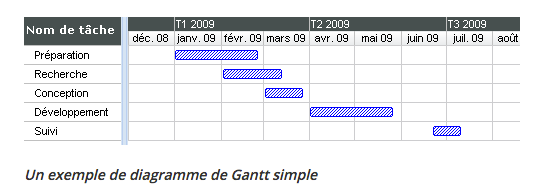
\includegraphics[keepaspectratio]{images/GANTT.png}}
\end{center}
\\
\href{https://lequartier.animafac.net/fiches-pratiques/outils-numeriques-structurer-projet-associatif/}{\emph{Source}}

\subsubsection{Roue de Deming (PCDA)}\label{roue-de-deming-pcda}

\begin{itemize}
\item
  Un cycle itératif pour l'amélioration continue :

  \begin{itemize}
  \tightlist
  \item
    Plan (planifier) : Définir les objectifs et les actions nécessaires.
  \item
    Do (faire) : Exécuter le plan.
  \item
    Check (vérifier) : Mesurer et analyser les résultats.
  \item
    Act (agir) : Ajuster et améliorer en fonction des retours.
  \end{itemize}
\item
  Utilisé pour garantir que chaque étape est maîtrisée et optimisée.
\end{itemize}

\begin{center}
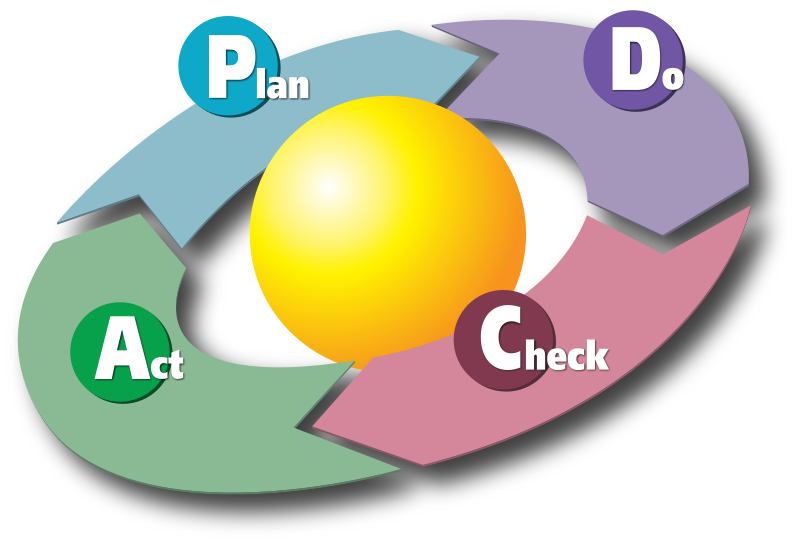
\includegraphics[width=5.20833in,height=\textheight,keepaspectratio]{images/PCDA.png}
\end{center}
\\
\href{https://web.archive.org/web/20210624065640/https://learn.saylor.org/mod/page/view.php?id=21134}{\emph{Source}}

\subsubsection{Les 0 Olympiques (Objectif
``Zéro'')}\label{les-0-olympiques-objectif-zuxe9ro}

\begin{itemize}
\item
  Inspiré du toyotisme, cela vise :

  \begin{itemize}
  \tightlist
  \item
    Zéro défaut : Produire sans erreur.
  \item
    Zéro pannes : Maintenir régulièrement pour éviter les pannes.
  \item
    Zéro papiers : Réduire les frais administratifs(monétaire et
    temporel).
  \item
    Zéro délais : Minimiser les retards.
  \item
    Zéro stocks : Éviter les surplus inutiles.
  \end{itemize}
\end{itemize}

\begin{center}
\pandocbounded{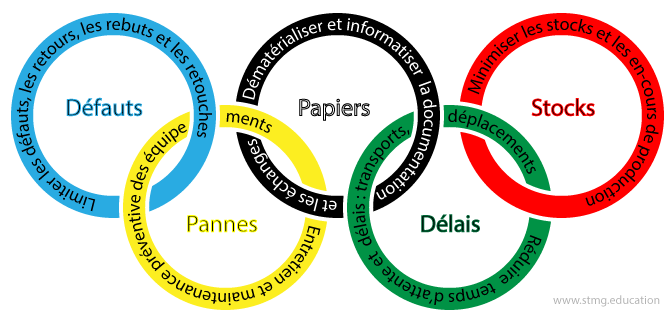
\includegraphics[keepaspectratio]{images/5-zeros.png}}
\end{center}
\\
\href{https://stmg.education/les-dicos/dico-management/zero.html}{\emph{Source}}

\subsubsection{Méthode des 5S (complément
toyotiste)}\label{muxe9thode-des-5s-compluxe9ment-toyotiste}

\begin{itemize}
\tightlist
\item
  Seiri (Trier), Seiton (Ranger), Seiso (Nettoyer), Seiketsu
  (Standardiser), Shitsuke (Soutenir).
\item
  Une méthode pour organiser efficacement les espaces de travail et
  garantir un environnement productif.
\end{itemize}

\subsubsection{Chemin critique (Critical Path
Method)}\label{chemin-critique-critical-path-method}

\begin{itemize}
\tightlist
\item
  Analyse des tâches pour identifier celles qui déterminent la durée
  totale du projet.
\item
  Cela permet de se concentrer sur les étapes les plus critiques pour
  respecter les délais.
\end{itemize}

\subsection{Une application, c'est quoi
?}\label{une-application-cest-quoi}

Une application est un programme informatique conçu pour répondre à un
besoin précis, comme envoyer des messages, faire des achats en ligne ou
gérer des données. Elle est utilisée par des utilisateurs via des
interfaces (smartphones, ordinateurs).

\subsubsection{Comment ça marche ?}\label{comment-uxe7a-marche}

\begin{itemize}
\item
  \textbf{Frontend (partie visible) :}\\
  C'est l'interface que vous voyez et utilisez (boutons, formulaires,
  pages web). Elle est conçue pour être intuitive et agréable à
  utiliser.
\item
  \textbf{Backend (partie invisible) :}\\
  C'est la ``machinerie'' qui fait fonctionner l'application. Elle
  traite les données, exécute les calculs et gère les demandes de
  l'utilisateur.
\item
  \textbf{Exemple :} Sur une page web d'achat en ligne, vous pouvez voir
  un bouton ``Commander'', parfaitement mis en valeur pour que vous
  puissiez cliquer dessus sans trop chercher (frontend), quand vous
  cliquerez sur ``Commander'', votre commande sera enregistrée et votre
  paiement validé (backend).
\end{itemize}

\subsubsection{Pourquoi une application
?}\label{pourquoi-une-application}

Une application est créée pour résoudre un problème ou simplifier une
tâche, c'est une solution qui répond à un besoin, par exemple :

\begin{itemize}
\item
  Commander un repas sans avoir à se déplacer.
\item
  Gérer des rendez-vous professionnels.
\item
  Analyser des données dans une entreprise.
\end{itemize}

\subsubsection{Penser design et
interface}\label{penser-design-et-interface}

Une application bien conçue doit :

\begin{itemize}
\item
  Être \textbf{simple à utiliser} : l'utilisateur ne doit pas se perdre
  ou être frustré.
\item
  Être \textbf{agréable visuellement} : des couleurs, polices et boutons
  clairs.
\item
  \textbf{S'adapter à tous les appareils} : ordinateurs, smartphones,
  tablettes (design ``responsive'').
\end{itemize}

La culture applicative, c'est comprendre qu'une application est une
combinaison entre ce que l'utilisateur voit (frontend) et la technologie
qui fonctionne en arrière-plan (backend), avec comme objectif de rendre
la vie plus simple et agréable grâce à un bon design et une utilité
claire.

\subsection{Rigueur est mère de réussite : le génie
logiciel}\label{rigueur-est-muxe8re-de-ruxe9ussite-le-guxe9nie-logiciel}

Pour atteindre ses objectifs de façon rigoureuse, il est possible
d'appliquer plusieurs concepts :

\begin{itemize}
\tightlist
\item
  Le \textbf{software engineering} (ou génie logiciel) est la discipline
  qui consiste à concevoir, développer, tester, et maintenir des
  logiciels de manière organisée et efficace.
\end{itemize}

\subsubsection{Conception structurée}\label{conception-structuruxe9e}

Avant de coder, on planifie comment le logiciel va fonctionner (quelles
sont ses fonctionnalités, sa structure). Cela inclut des étapes comme la
création de diagrammes ou l'écriture d'un cahier des charges.

\subsubsection{Bonnes pratiques de code}\label{bonnes-pratiques-de-code}

Écrire du code de qualité est crucial pour garantir que le logiciel soit
lisible, réutilisable, et facile à maintenir. Voici quelques bonnes
pratiques :

\begin{itemize}
\item
  \textbf{DRY (Don't Repeat Yourself)} : Éviter de dupliquer le code ;
  si une fonctionnalité doit être réutilisée, elle doit être écrite une
  seule fois et utilisée partout.
\item
  \textbf{KISS (Keep It Simple, Stupid)} : Rendre le code aussi simple
  que possible pour éviter des solutions inutiles ou complexes.
\item
  \textbf{SOLID} : Ensemble de principes qui facilitent la conception
  orientée objet :

  \begin{itemize}
  \item
    \textbf{S} : Single Responsibility Principle (chaque classe doit
    avoir une seule responsabilité).
  \item
    \textbf{O} : Open/Closed Principle (le code doit être ouvert à
    l'extension mais fermé à la modification).
  \item
    \textbf{L} : Liskov Substitution Principle (les sous-classes doivent
    pouvoir remplacer leurs classes parentes).
  \item
    \textbf{I} : Interface Segregation Principle (les interfaces doivent
    être spécifiques à un usage).
  \item
    \textbf{D} : Dependency Inversion Principle (les modules de haut
    niveau ne doivent pas dépendre de modules de bas niveau, mais des
    abstractions).
  \end{itemize}
\item
  \href{https://peps.python.org/pep-0008/}{\textbf{PEP8}}
  \textbf{(Python Enhancement Proposal)} : Un guide de style pour écrire
  du code Python clair et lisible, couvrant des aspects comme les
  indentations, les noms de variables, et les espaces.
\end{itemize}

\subsubsection{Structurer un projet}\label{structurer-un-projet}

Un projet bien structuré est essentiel pour être déployable en
production et maintenable dans le temps. Cela inclut :

\begin{itemize}
\item
  Une organisation claire des fichiers et des dossiers.
\item
  Une séparation entre le code source, les tests, et la configuration.
\item
  Une documentation complète expliquant le fonctionnement du logiciel et
  les étapes pour contribuer au projet.
\end{itemize}

\subsubsection{Tests et qualité}\label{tests-et-qualituxe9}

Tester un logiciel garantit qu'il fonctionne correctement et répond aux
besoins.

\begin{itemize}
\tightlist
\item
  \textbf{Tests unitaires :} Vérifient des petites parties du code (ex.
  une seule fonction).
\item
  \textbf{Tests d'intégration :} Vérifient que différentes parties du
  code fonctionnent ensemble.
\item
  \textbf{Automatisation des tests :} Les outils comme pytest (en
  Python) permettent d'automatiser les tests pour gagner du temps.
\end{itemize}

Pour renforcer la qualité, on utilise des linters (ex. \emph{pylint,
flake8}) qui analysent le code pour repérer les erreurs de style ou de
logique avant qu'elles ne causent des problèmes.

\subsubsection{Collaboration et gestion des
versions}\label{collaboration-et-gestion-des-versions}

Le développement logiciel est souvent un travail d'équipe. Des outils
comme Git permettent de :

\begin{itemize}
\tightlist
\item
  Gérer différentes versions du code.
\item
  Suivre l'historique des modifications.
\item
  Collaborer efficacement en évitant les conflits entre les
  contributions des développeurs.
\end{itemize}

\subsubsection{Adopter des patterns de
design}\label{adopter-des-patterns-de-design}

Les design patterns sont des solutions éprouvées pour résoudre des
problèmes fréquents de conception logicielle. Par exemple :

\begin{itemize}
\tightlist
\item
  \textbf{Singleton :} Garantir qu'une classe n'ait qu'une seule
  instance.
\item
  \textbf{Factory :} Centraliser la création d'objets complexes.
\item
  \textbf{Observer :} Réagir aux changements d'état dans un système.
\end{itemize}

\subsubsection{Le Zen of Python}\label{le-zen-of-python}

Une philosophie de développement Python, illustrée par des principes
comme :

\begin{itemize}
\tightlist
\item
  ``Beautiful is better than ugly'' (un code lisible est préférable).
\item
  ``Simple is better than complex'' (la simplicité est essentielle).
\item
  ``Errors should never pass silently'' (les erreurs doivent être
  explicites).
\end{itemize}

Ces pratiques sont essentielles pour concevoir des logiciels efficaces,
maintenables et collaboratifs.\\
Pour conclure, le génie logiciel, c'est comme construire une maison : il
faut des plans solides, des matériaux adaptés (le code), un contrôle
qualité (tests), et un design qui facilite les rénovations futures
(maintenance).

\subsection{Commencer sur de bonnes bases :
Python}\label{commencer-sur-de-bonnes-bases-python}

\subsubsection{Les fonctions}\label{les-fonctions}

Une fonction est un bloc de code qui effectue une tâche spécifique. Vous
pouvez la réutiliser plusieurs fois.\\
Exemple :

\begin{Shaded}
\begin{Highlighting}[]
\KeywordTok{def}\NormalTok{ dire\_bonjour(nom):}
    \ControlFlowTok{return} \SpecialStringTok{f"Bonjour, }\SpecialCharTok{\{}\NormalTok{nom}\SpecialCharTok{\}}\SpecialStringTok{ !"}

\BuiltInTok{print}\NormalTok{(dire\_bonjour(}\StringTok{"Alice"}\NormalTok{))}
\end{Highlighting}
\end{Shaded}

Ici, la fonction \emph{dire\_bonjour} prend un nom et retourne un
message personnalisé.

\subsubsection{Tests unitaires}\label{tests-unitaires}

Les tests unitaires permettent de vérifier qu'une partie précise de
votre code (comme une fonction) fonctionne correctement.\\
Exemple avec la bibliothèque unittest :

\begin{Shaded}
\begin{Highlighting}[]
\ImportTok{import}\NormalTok{ unittest}

\KeywordTok{def}\NormalTok{ addition(a, b):}
    \ControlFlowTok{return}\NormalTok{ a }\OperatorTok{+}\NormalTok{ b}

\KeywordTok{class}\NormalTok{ TestAddition(unittest.TestCase):}
    \KeywordTok{def}\NormalTok{ test\_positif(}\VariableTok{self}\NormalTok{):}
        \VariableTok{self}\NormalTok{.assertEqual(addition(}\DecValTok{2}\NormalTok{, }\DecValTok{3}\NormalTok{), }\DecValTok{5}\NormalTok{)}

\ControlFlowTok{if} \VariableTok{\_\_name\_\_} \OperatorTok{==} \StringTok{"\_\_main\_\_"}\NormalTok{:}
\NormalTok{    unittest.main()}
\end{Highlighting}
\end{Shaded}

Cela permet de détecter les erreurs dès que le code change.

\subsubsection{Objets et classes (Programmation orientée
objet)}\label{objets-et-classes-programmation-orientuxe9e-objet}

Python permet de créer des classes, des ``modèles'' pour structurer vos
données et comportements.

Exemple :

\begin{Shaded}
\begin{Highlighting}[]
\KeywordTok{class}\NormalTok{ Animal:}
    \KeywordTok{def} \FunctionTok{\_\_init\_\_}\NormalTok{(}\VariableTok{self}\NormalTok{, nom):}
        \VariableTok{self}\NormalTok{.nom }\OperatorTok{=}\NormalTok{ nom}

    \KeywordTok{def}\NormalTok{ parler(}\VariableTok{self}\NormalTok{):}
        \ControlFlowTok{return} \SpecialStringTok{f"}\SpecialCharTok{\{}\VariableTok{self}\SpecialCharTok{.}\NormalTok{nom}\SpecialCharTok{\}}\SpecialStringTok{ fait un bruit."}

\NormalTok{chien }\OperatorTok{=}\NormalTok{ Animal(}\StringTok{"Rex"}\NormalTok{)}
\BuiltInTok{print}\NormalTok{(chien.parler())  }\CommentTok{\# Rex fait un bruit.}
\end{Highlighting}
\end{Shaded}

Une classe regroupe des données (\emph{nom}) et des comportements
(\emph{parler}).

\subsubsection{Environnements virtuels (avec
Docker)}\label{environnements-virtuels-avec-docker}

Un \textbf{environnement virtuel} permet d'isoler les dépendances
(bibliothèques, versions de Python) d'un projet pour éviter les conflits
avec d'autres projets.

\begin{itemize}
\tightlist
\item
  Avec Python :
\end{itemize}

\begin{Shaded}
\begin{Highlighting}[]
\ExtensionTok{python} \AttributeTok{{-}m}\NormalTok{ venv mon\_env}
\BuiltInTok{source}\NormalTok{ mon\_env/bin/activate  }\CommentTok{\# Active l\textquotesingle{}environnement}
\ExtensionTok{pip}\NormalTok{ install numpy            }\CommentTok{\# Installe une bibliothèque uniquement pour cet environnement}
\end{Highlighting}
\end{Shaded}

\begin{itemize}
\tightlist
\item
  Avec Docker (outil pour des environnements plus complexes) :\\
  Docker crée des conteneurs, qui isolent tout un système (pas seulement
  Python).\\
  Exemple d'un fichier Dockerfile :
\end{itemize}

\begin{Shaded}
\begin{Highlighting}[]
\KeywordTok{FROM}\NormalTok{ python:3.9}
\KeywordTok{WORKDIR}\NormalTok{ /app}
\KeywordTok{COPY}\NormalTok{ . .}
\KeywordTok{RUN} \ExtensionTok{pip}\NormalTok{ install }\AttributeTok{{-}r}\NormalTok{ requirements.txt}
\KeywordTok{CMD}\NormalTok{ [}\StringTok{"python"}\NormalTok{, }\StringTok{"main.py"}\NormalTok{]}
\end{Highlighting}
\end{Shaded}

Cela garantit que votre application fonctionnera partout de la même
manière.

En résumé, maîtriser ces bases vous aide à écrire un code réutilisable,
fiable, et bien organisé, tout en travaillant dans des environnements
adaptés.

\subsection{Plus on est de pro, plus on
rit}\label{plus-on-est-de-pro-plus-on-rit}

De votre rôle de professionnel de la donnée, dans les projets, vous
serez amenez à travailler avec divers métiers, il est important de
comprendre les fonctionnements et les missions de vos futurs
collaborateurs.\\
Parmi ces individus avec lesquels vous allez collaborer fréquemment :

\textbf{Le Product Manager (PM)}

\begin{itemize}
\tightlist
\item
  \textbf{Rôle :} Définit la stratégie et les objectifs d'un produit ou
  d'un projet en s'appuyant sur des analyses de données.
\item
  \textbf{Collaboration :} Il travaille avec des data scientists et data
  analysts pour comprendre les tendances utilisateurs et prendre des
  décisions stratégiques basées sur les données.
\end{itemize}

\textbf{Le Développeur Backend}

\begin{itemize}
\tightlist
\item
  \textbf{Rôle :} Construit les systèmes qui collectent et rendent
  accessibles les données (APIs, bases de données).
\item
  \textbf{Collaboration :} Il travaille avec les data engineers pour
  intégrer les pipelines de données et avec les data scientists pour
  fournir les données nécessaires à leurs analyses.
\end{itemize}

\textbf{Le Développeur Frontend}

\begin{itemize}
\tightlist
\item
  \textbf{Rôle :} Développe des interfaces utilisateur (sites web,
  tableaux de bord, applications) pour visualiser ou interagir avec les
  données.
\item
  \textbf{Collaboration :} Il travaille avec des data analysts et des
  business intelligence analysts pour présenter les données de manière
  compréhensible et esthétique.
\end{itemize}

\textbf{Le Spécialiste en Cybersécurité}

\begin{itemize}
\tightlist
\item
  \textbf{Rôle :} Protège les systèmes et les données contre les
  attaques et les intrusions.
\item
  \textbf{Collaboration :} Il s'associe à des data governance
  specialists et des data engineers pour sécuriser les pipelines de
  données et garantir la conformité aux régulations.
\end{itemize}

\textbf{Le Cloud Architect}

\begin{itemize}
\tightlist
\item
  \textbf{Rôle :} Conçoit les infrastructures cloud pour héberger et
  traiter les données à grande échelle.
\item
  \textbf{Collaboration :} Il travaille avec des data engineers et des
  big data engineers pour s'assurer que les systèmes cloud répondent aux
  besoins de stockage et de calcul.
\end{itemize}

\textbf{Le Consultant en Transformation Digitale}

\begin{itemize}
\tightlist
\item
  \textbf{Rôle :} Aide les entreprises à intégrer les données dans leurs
  processus décisionnels et leurs outils numériques.
\item
  \textbf{Collaboration :} Il collabore avec des chief data officers,
  data scientists et business intelligence analysts pour orienter les
  projets.
\end{itemize}

\textbf{L'UX Designer (Designer d'expérience utilisateur)}

\begin{itemize}
\tightlist
\item
  \textbf{Rôle :} Conçoit des interfaces utilisateur et des parcours
  fluides en se basant sur les données utilisateurs.
\item
  \textbf{Collaboration :} Il utilise les insights des data analysts et
  des product managers pour optimiser l'expérience utilisateur.
\end{itemize}

\textbf{L'Ingénieur DevOps}

\begin{itemize}
\tightlist
\item
  \textbf{Rôle :} Automatise et optimise le déploiement des
  applications, y compris les modèles d'apprentissage automatique ou les
  systèmes de traitement de données.
\item
  \textbf{Collaboration :} Il travaille avec les machine learning
  engineers et data engineers pour déployer les solutions en production.
\end{itemize}

\textbf{L'Analyste Marketing}

\begin{itemize}
\tightlist
\item
  \textbf{Rôle :} Utilise les données pour mesurer l'efficacité des
  campagnes publicitaires et comprendre le comportement des clients.
\item
  \textbf{Collaboration :} Il collabore avec les data analysts et les
  business intelligence analysts pour extraire et interpréter les
  métriques marketing.
\end{itemize}

\textbf{Le Responsable de la Conformité (Compliance Officer)}

\begin{itemize}
\tightlist
\item
  \textbf{Rôle :} S'assure que l'entreprise respecte les lois et
  régulations liées aux données (comme le RGPD).
\item
  \textbf{Collaboration :} Il travaille avec les data governance
  specialists pour encadrer l'usage des données de manière légale et
  éthique.
\end{itemize}

Ces métiers feront certainement parti de l'écosystème auquel vous
appartiendrez et contribuerons à vos projets de près ou de loin.




\end{document}
